\documentclass[12pt,a4paper]{paper}
\usepackage[utf8]{inputenc}
\usepackage[english]{babel}
\usepackage{amsmath}
\usepackage{enumitem}
\usepackage{amsfonts}
\usepackage{amssymb}
\usepackage[left=2cm,right=2cm,top=2cm,bottom=2cm]{geometry}
\usepackage{Sweave}
\begin{document}
\title{STAT646 - Homework 3\\\small{Daniel Osorio - dcosorioh@tamu.edu\\Department of Veterinary Integrative Biosciences\\Texas A\&M University}}
\maketitle
\Sconcordance{concordance:Osorio_Daniel_HW3.tex:Osorio_Daniel_HW3.Rnw:%
1 8 1 1 0 9 1 4 0 1 3 1 4 3 0 1 2 1 0 5 1 1 3 2 0 1 1 1 5 4 0 1 2 1 0 1 %
3 6 0 1 2 2 1}

\begin{enumerate}
\item Read the minfi tutorial: \\https://www.bioconductor.org/help/course-materials/2015/BioC2015/methylation450k.html
\item Read the Breacher analysis2.pdf. Take the RGset data, the phenotype data (uploaded at eCampus) and perform the following steps:
\begin{enumerate}
\item Normalize the data using SWAN normalization.
\begin{Schunk}
\begin{Sinput}
> library(minfi)
> library(limma)
\end{Sinput}
\end{Schunk}
\begin{Schunk}
\begin{Sinput}
> load("rgset_breacher.Rdata")
> phenoData <- pData(valid_RGset)
> bL_rgSet <- valid_RGset[,grepl("1$",phenoData$Sample_Name)]
> colnames(bL_rgSet) <- phenoData[grepl("1$",phenoData[,1]),1]
> bL_rgSet <- bL_rgSet[,!colnames(bL_rgSet) %in% "3X01_1"]
> # Normalization
> mSet <- preprocessRaw(valid_RGset)
> colnames(mSet) <- phenoData[,1]
> mSet_illlumina <- preprocessIllumina(rgSet = valid_RGset, 
+                                      bg.correct = TRUE, 
+                                      normalize = "controls")
> mSet_swan <- preprocessSWAN(valid_RGset, mSet_illlumina)
> colnames(mSet_swan) <- phenoData[,1]
\end{Sinput}
\end{Schunk}
\begin{Schunk}
\begin{Sinput}
> par(mfrow=c(1,2), mar = c(3,3,1,1), mgp=c(1.5,0.5,0))
> plotBetasByType(mSet[,1], main = "RAW")
> plotBetasByType(mSet_swan[,1], main = "SWAN")
\end{Sinput}
\end{Schunk}
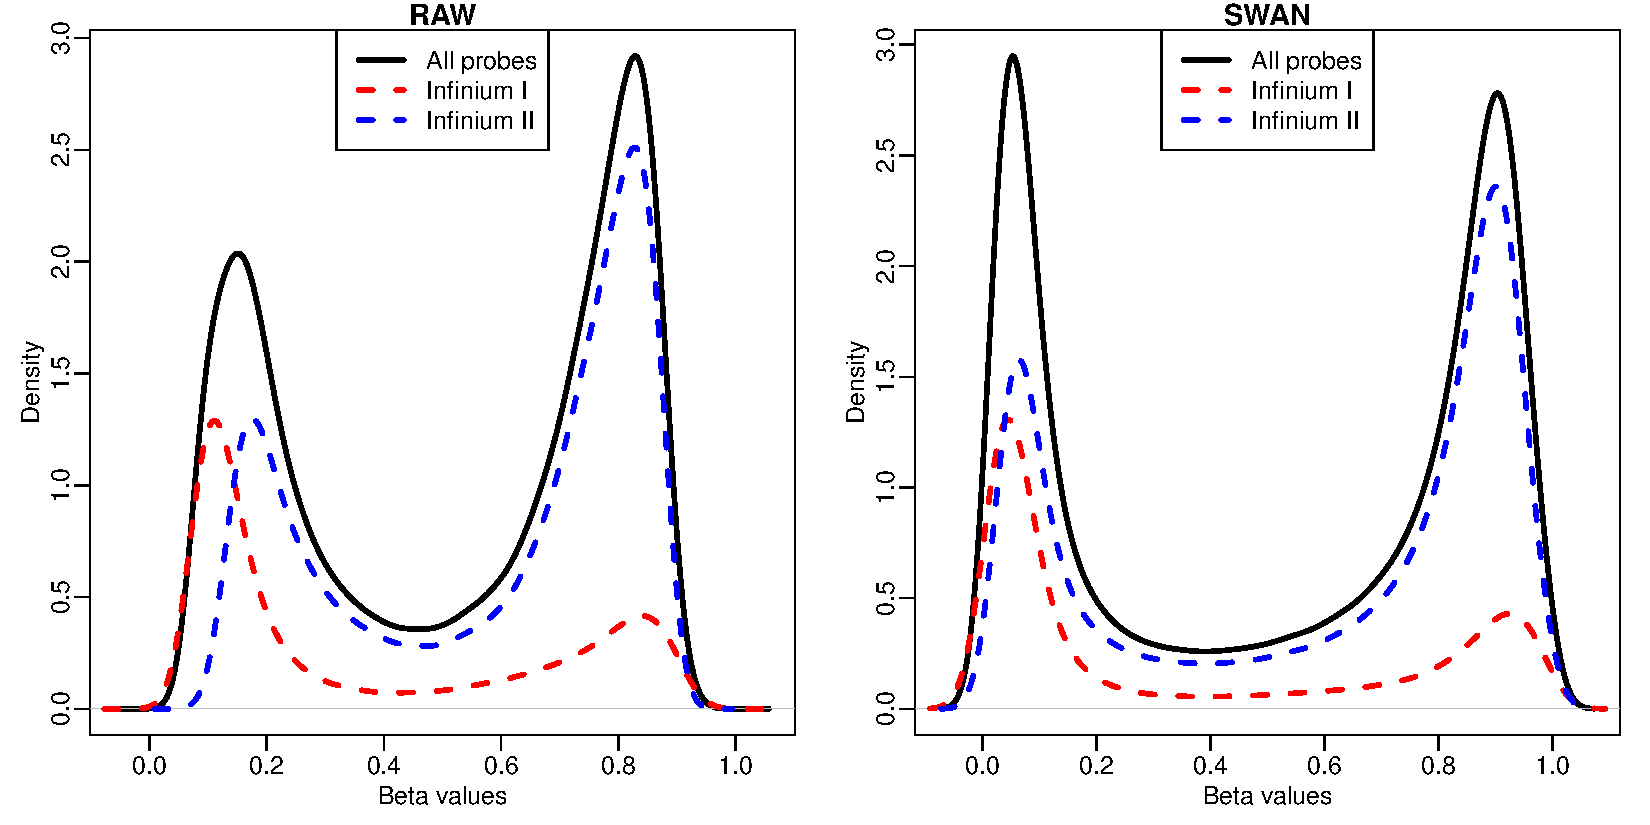
\includegraphics{Osorio_Daniel_HW3-003}
\item Recreate all the plots from the Breacher\_analysis2.pdf file.
\begin{Schunk}
\begin{Sinput}
> bL <- phenoData[phenoData[,1] %in% colnames(bL_rgSet),]
> colnames(bL)[6] <- "Breaches"
> bL$Breaches[bL$Breaches %in% c("400+", "200-399")] <- "200+"
> newLevels <- c("0", "1-9", "10-39", "40-99", "100-199", "200+")
> bL$Breaches <- factor(x = bL$Breaches, levels = newLevels)
\end{Sinput}
\end{Schunk}
\begin{Schunk}
\begin{Sinput}
> par(mar=c(3,3,2,1), mgp = c(1.5,0.5,0), mfrow = c(1,2))
> plot(x = bL$Breaches, main = "# Breaches", xlab = "Categories", 
+      ylab = "Breaches", las = 1)
> pie(x = c('65.625%' = 2100/32,'34.375%'=1100/32), 
+     col = c("red", "skyblue"))
> legend("topright", legend = c("<39", ">39"), 
+        fill = c("red", "skyblue"), bty = "n")
\end{Sinput}
\end{Schunk}
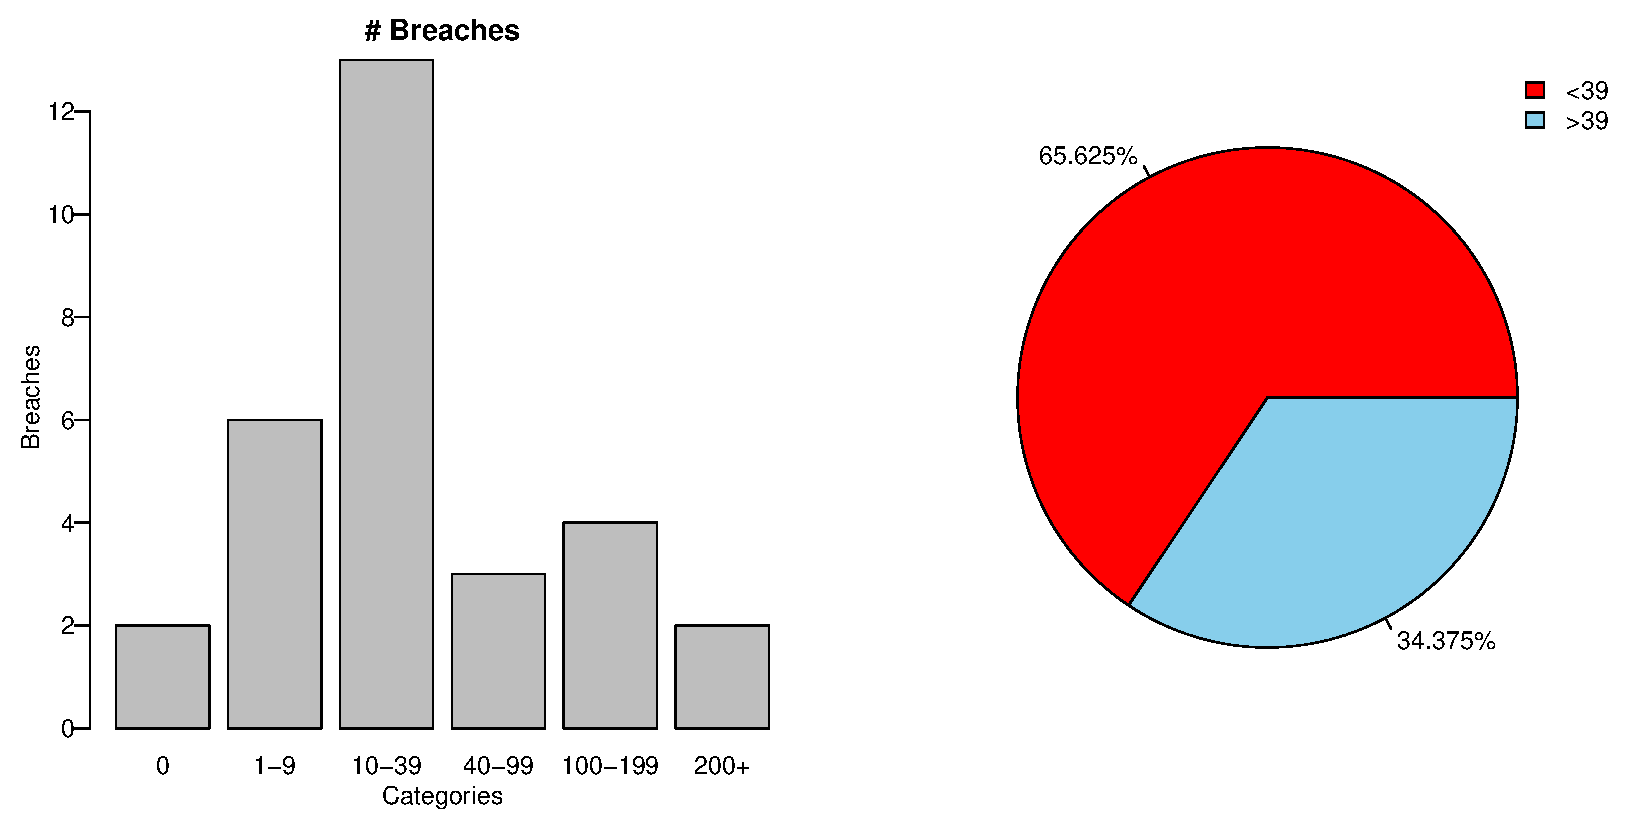
\includegraphics{Osorio_Daniel_HW3-005}
\begin{Schunk}
\begin{Sinput}
> TB <- ifelse(bL$num_prior_TBIs > 0, yes = "yes", no = "no")
> barplot(height = table(TB, bL$Breaches), col = c("red", "black"))
> legend("topright", legend = c("TBI = YES", "TBI = NO"), 
+        fill = c("black", "red"), bty = "n")
\end{Sinput}
\end{Schunk}
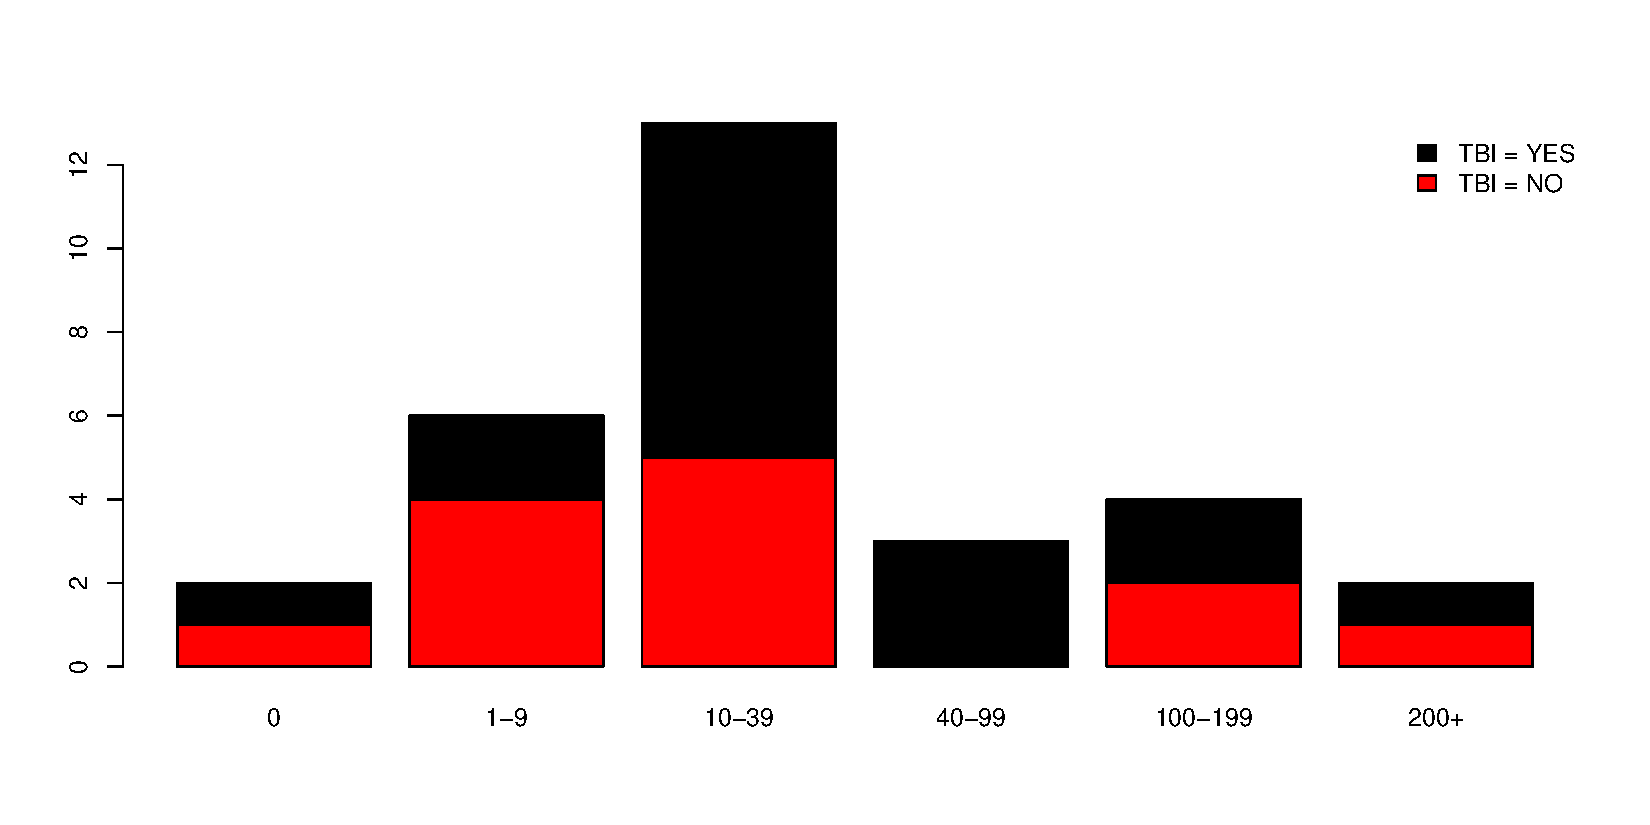
\includegraphics{Osorio_Daniel_HW3-006}

\begin{Schunk}
\begin{Sinput}
> rSet <- ratioConvert(mSet, what = "both", keepCN = TRUE)
> betaRaw <- getBeta(rSet)
> rSet <- mapToGenome(rSet)
> xIndex <- which(seqnames(rSet) == "chrX")
> yIndex <- which(seqnames(rSet) == "chrY")
> xMed <- matrixStats::colMedians(betaRaw[xIndex,], na.rm=TRUE)
> yMed <- matrixStats::colMedians(betaRaw[yIndex,], na.rm=TRUE)
> par(mar=c(5,3,1,1))
> plot(c(1,nrow(phenoData)),c(-1,1),type="n",axes=FALSE,xlab="",ylab="",
+ main="Median beta values for Chromosomes X and Y")
> points(x = seq_len(nrow(phenoData)),y = xMed, pch=16)
> points(x = seq_len(nrow(phenoData)),y = -yMed, pch=20)
> axis(1,1:nrow(phenoData), phenoData[,1] ,las=2,cex=0.6)
> at <- seq(0,1,0.2)
> axis(2,at = c(at,-at[-1]),labels = c(at,at[-1]))
> abline(h=0)
> mtext("chrX median beta",2,line=2,at=0.5,adj=0.5)
> mtext("ChrY median beta",2,line=2,at=-0.5,adj=0.5)
> box()
> segments(c(1:nrow(phenoData)),y0=-yMed,y1=xMed)
\end{Sinput}
\end{Schunk}
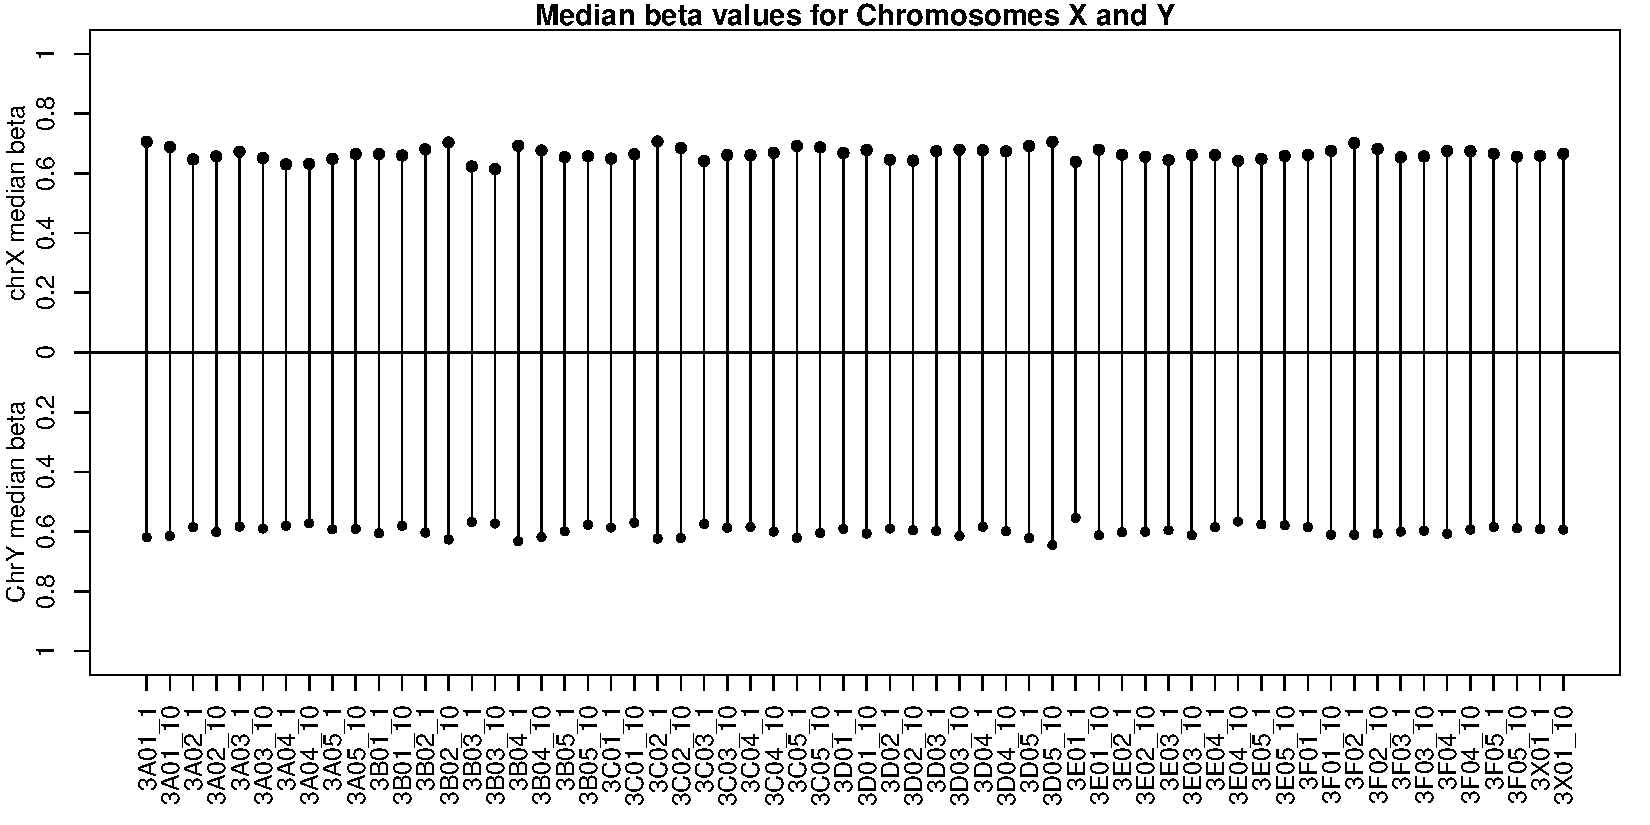
\includegraphics{Osorio_Daniel_HW3-007}

\begin{Schunk}
\begin{Sinput}
> SNPs <- getSnpBeta(valid_RGset)
> colnames(SNPs) <- phenoData$Sample_Name
> dMatrix <- dist(t(SNPs), method = "manhattan")
> hC <- hclust(dMatrix, method = "single")
> plot(hC)
\end{Sinput}
\end{Schunk}
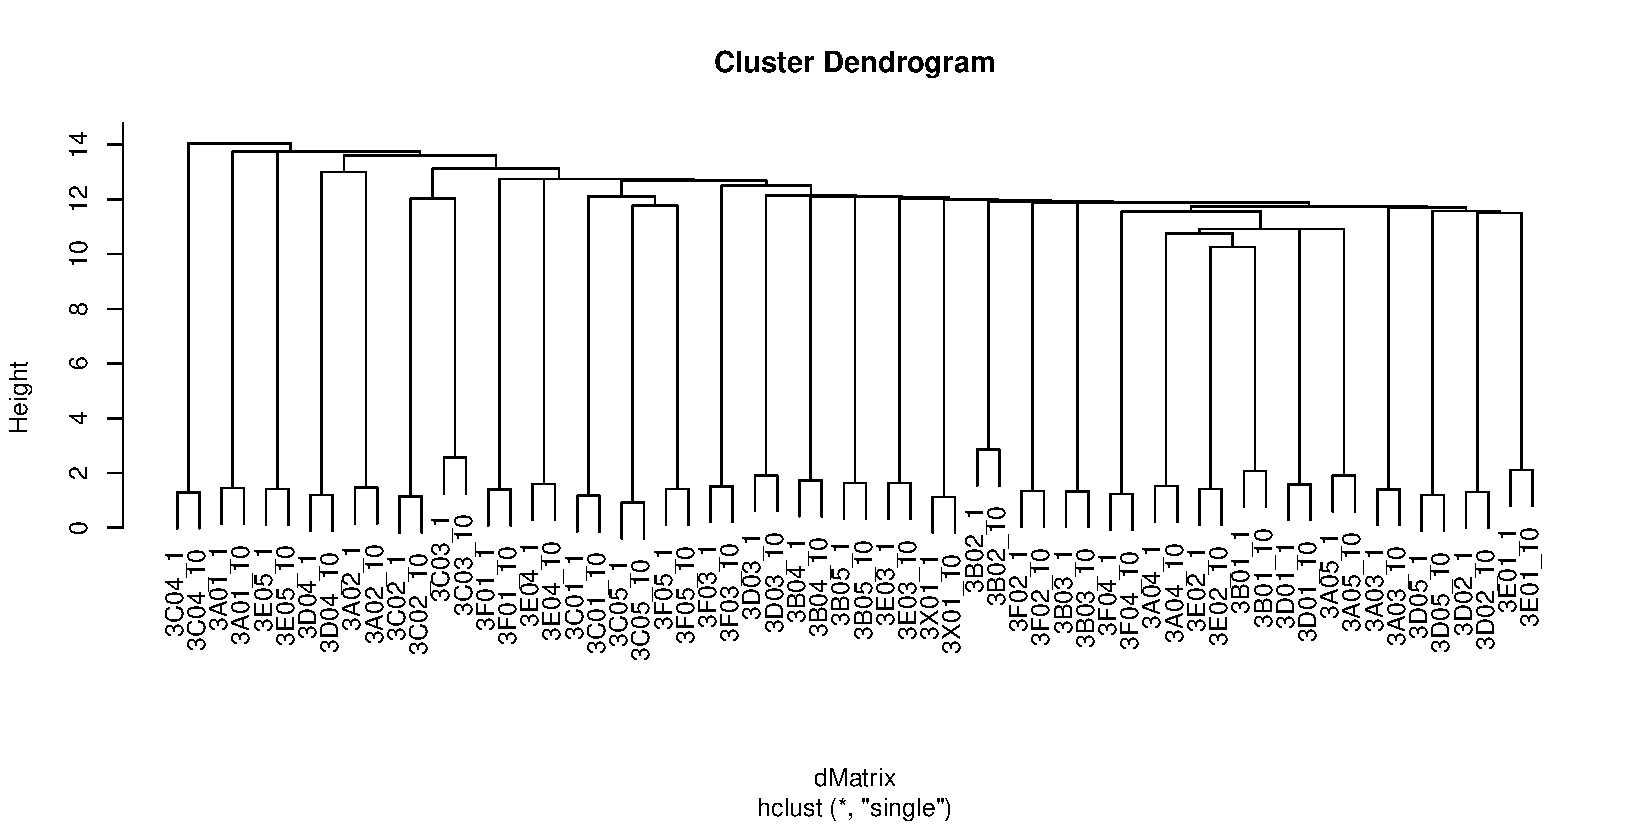
\includegraphics{Osorio_Daniel_HW3-008}

\begin{Schunk}
\begin{Sinput}
> detP <- detectionP(bL_rgSet)
> selectedP <- rowSums(detP < 0.01) == ncol(bL_rgSet)
> mSet_swan <- mSet_swan[selectedP,colnames(bL_rgSet)]
> beta_bL <- getBeta(mSet_swan)
> Mval_baseline <-getM(mSet_swan)
> career <- ifelse(as.numeric(bL$Breaches) > 2, yes = "high", no = "low")
> TB <- ifelse(bL$num_prior_TBIs > 0, yes = "yes", no = "no")
> historyTBI <- factor(TB,levels=c("yes","no"))
> design <- model.matrix(~bL$age + as.factor(career) + historyTBI)
> fit<- lmFit(Mval_baseline,design)
> fit.reduced <- eBayes(fit)
\end{Sinput}
\end{Schunk}

\begin{Schunk}
\begin{Sinput}
> top_breacher<-topTable(fit.reduced,coef=3,number=dim(Mval_baseline)[1])
> fc_breacher<-top_breacher$logFC
> fcbreacherplus<-fc_breacher[fc_breacher>0]
> fcbreacherminus<-abs(fc_breacher[fc_breacher<=0])
> hP <- hist(fcbreacherplus, breaks = 25, plot = FALSE)
> hM <- hist(fcbreacherminus, breaks = 25, plot= FALSE)
> hM$counts <- -1 * hM$counts
> yLim <- c(min(hM$counts,hP$counts),max(hM$counts,hP$counts))
> plot(hP,ylim=yLim, xlab = "methylation M-value difference", 
+      ylab = "# of CpGs", main = "Breach: low vs high",col = "red")
> plot(hM,ylim=yLim, col = "blue", add = TRUE)
\end{Sinput}
\end{Schunk}
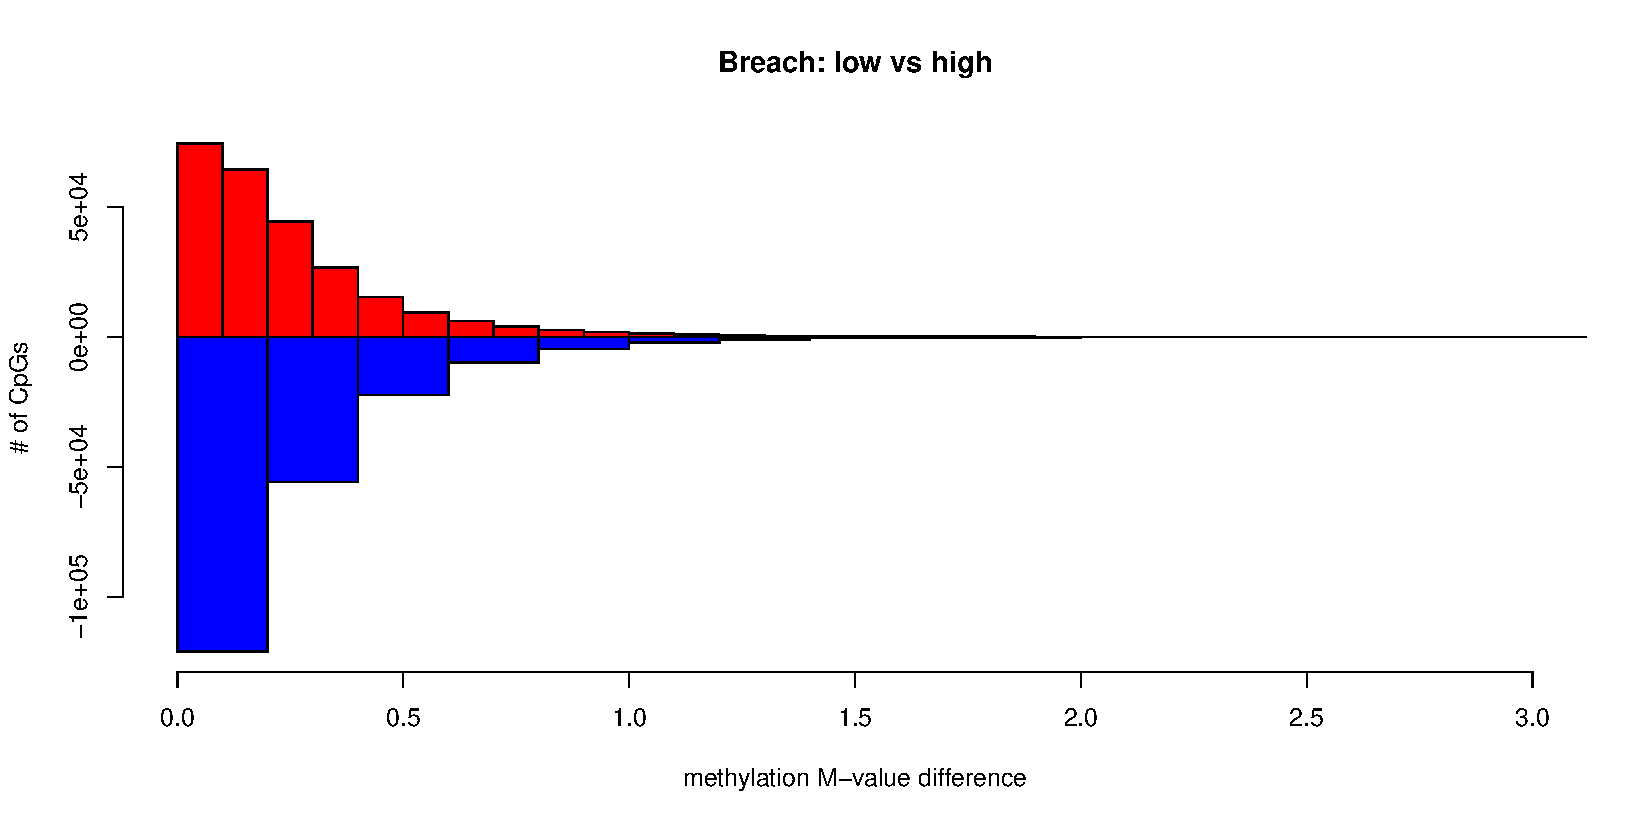
\includegraphics{Osorio_Daniel_HW3-010}

\begin{Schunk}
\begin{Sinput}
> mean_beta <- apply(beta_bL,2,mean)
> boxplot(mean_beta~career, col=c("gold","darkgreen"),
+         xlab="", ylab="beta values")
\end{Sinput}
\end{Schunk}
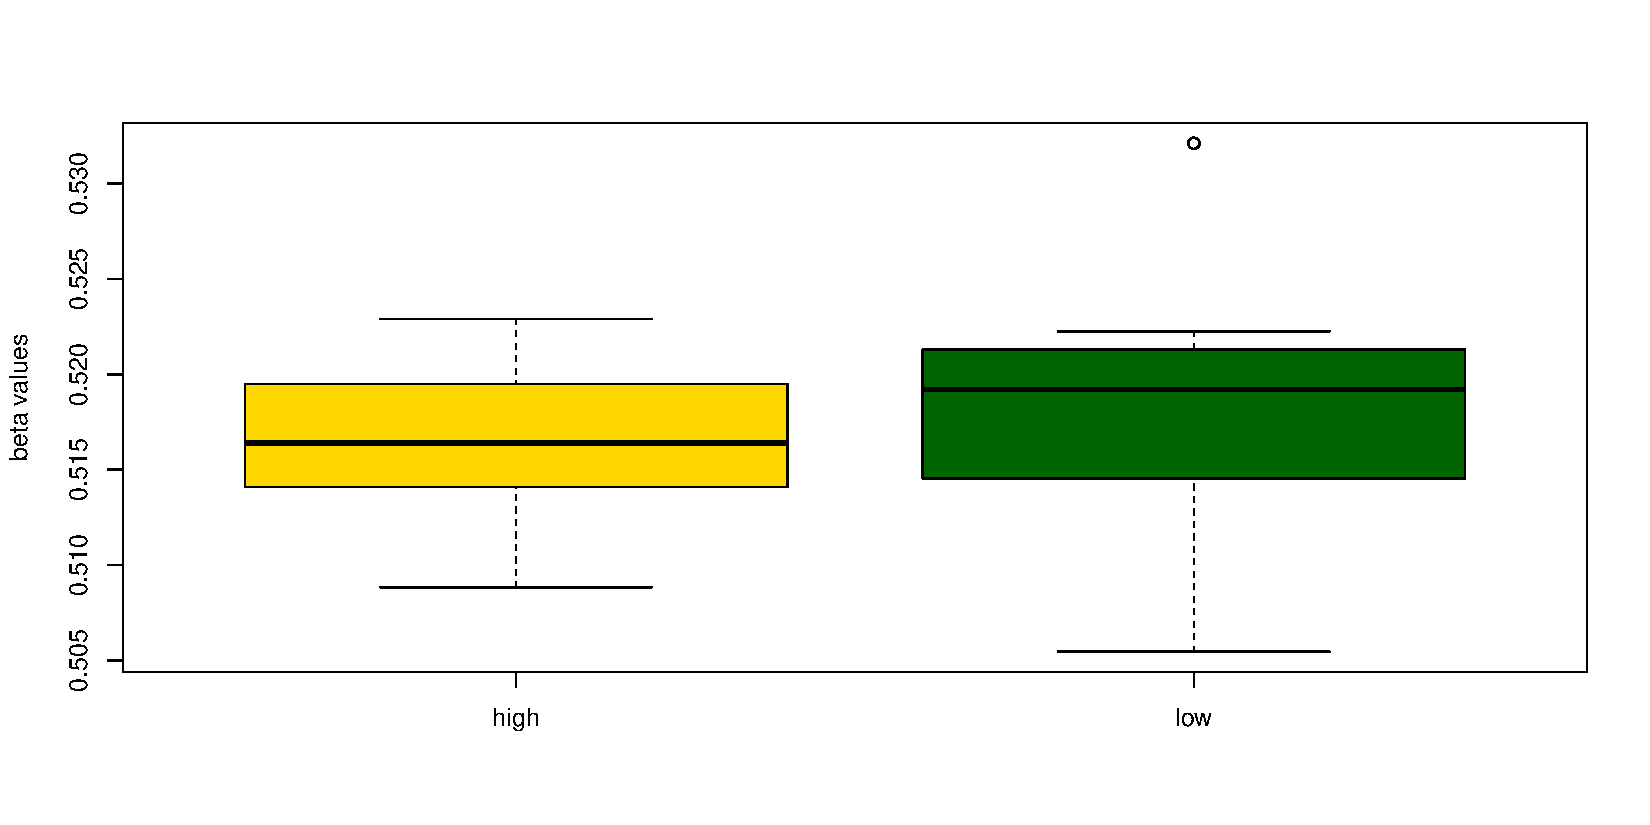
\includegraphics{Osorio_Daniel_HW3-011}

\begin{Schunk}
\begin{Sinput}
> plot(top_breacher$logFC, -log10(top_breacher$P.Value),
+      xlab="", ylab="-log10 p-value")
> abline(a=-log10(0.05), b=0, col="red")
\end{Sinput}
\end{Schunk}
\includegraphics{Osorio_Daniel_HW3-012}

\begin{Schunk}
\begin{Sinput}
> top_TBI<-topTable(fit.reduced,coef=4,number=dim(Mval_baseline)[1])
> fc_TBI<-top_TBI$logFC
> fcTBIplus<-fc_TBI[fc_TBI>0]
> fcTBIminus<-abs(fc_TBI[fc_TBI<=0])
> hP <- hist(fcTBIplus, breaks = 25, plot = FALSE)
> hM <- hist(fcTBIminus, breaks = 25, plot = FALSE)
> hM$counts <- -1 * hM$counts
> yLim <- c(min(hP$counts, hM$counts), max(hP$counts, hM$counts))
> plot(hP, ylim=yLim, xlab = "methylation M-value difference", 
+      ylab = "# of CpGs", main = "TBI: no vs yes",col = "red")
> plot(hM, ylim=yLim, add=TRUE, col = "blue")
\end{Sinput}
\end{Schunk}
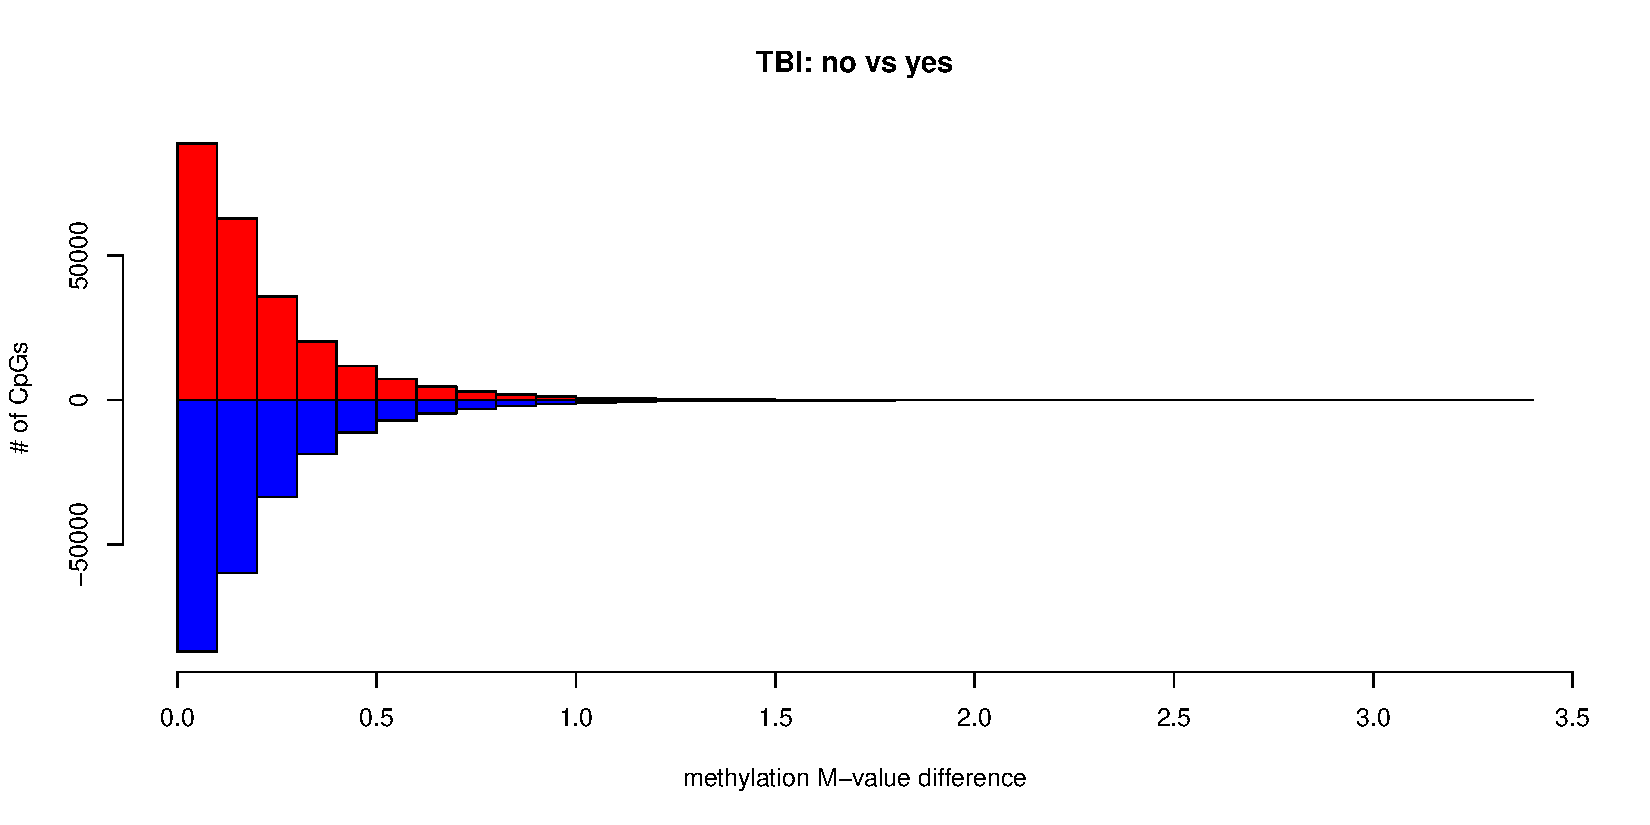
\includegraphics{Osorio_Daniel_HW3-013}

\begin{Schunk}
\begin{Sinput}
> annotation <- getAnnotation(bL_rgSet)
> positioninfo <- annotation$UCSC_RefGene_Group
> probename<-annotation$Name
> selected_probe <- which(probename %in% probename)
> position_selected <- positioninfo[selected_probe]
> countTSS <- sum(grepl("TSS",position_selected))
> count5UTR <- sum(grepl("5'UTR",position_selected))
> countbody <- sum(grepl("Body",position_selected))
> countexon <- sum(grepl("1stExon",position_selected))
> cate = c("TSS","body","1stExon","5'UTR");
> cnt <- c(countTSS,countbody,countexon,count5UTR)
> names(cnt) <- cate
> barplot(cnt, xlab="categories of region", 
+         ylab="",main="Barplot for regions")
\end{Sinput}
\end{Schunk}
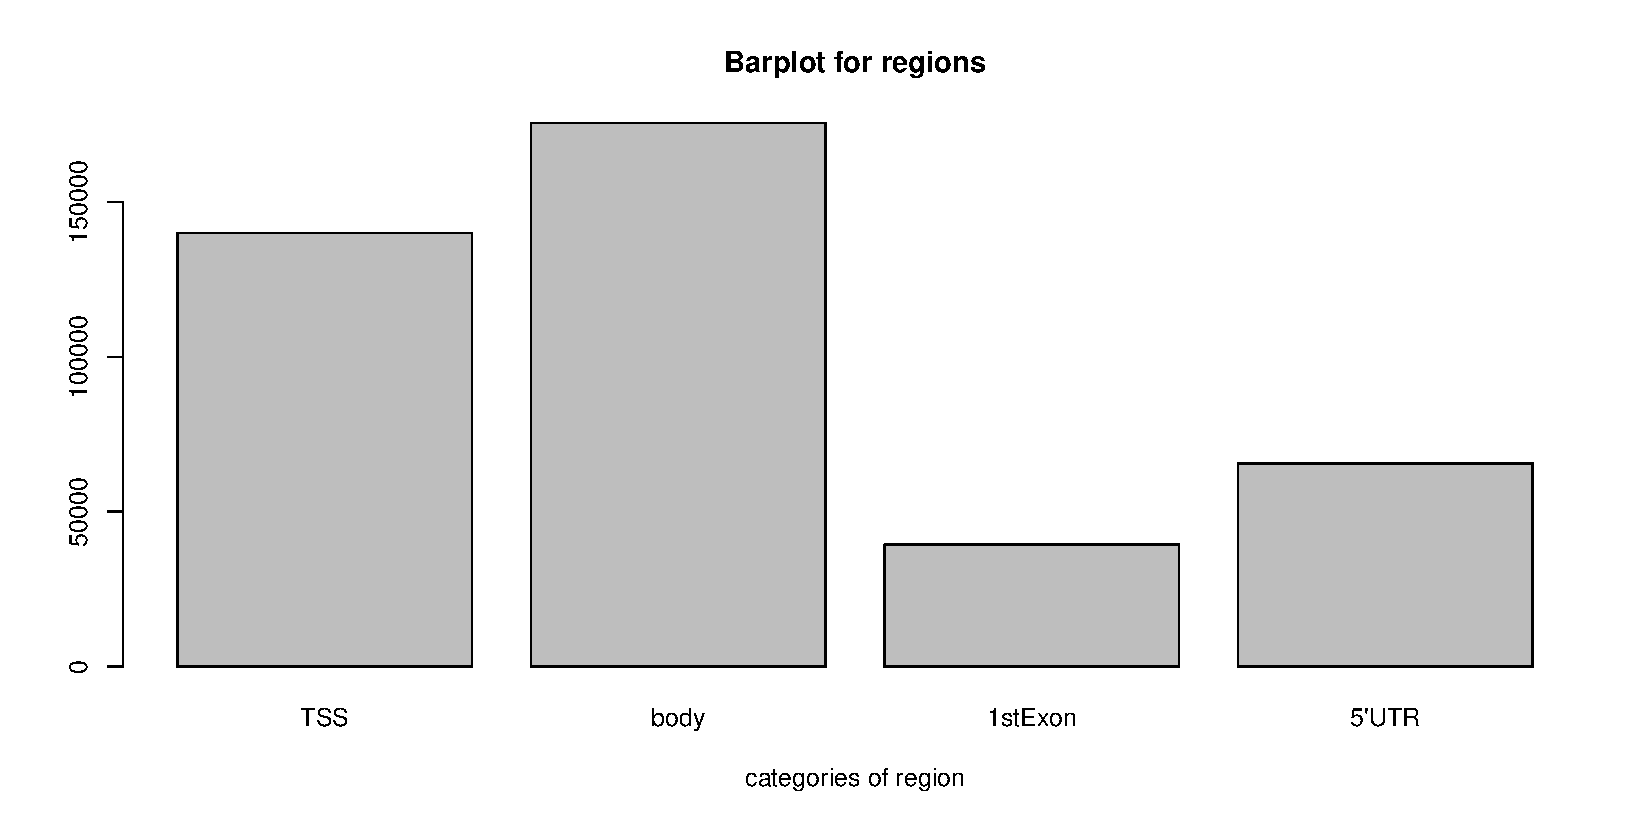
\includegraphics{Osorio_Daniel_HW3-014}

\begin{Schunk}
\begin{Sinput}
> Islandinfo<-annotation$Relation_to_Island
> Islandinfo_selected<-Islandinfo[selected_probe]
> countIsland=sum(grepl("Island",Islandinfo_selected))
> countNShelf=sum(grepl("N_Shelf",Islandinfo_selected))
> countNShore=sum(grepl("N_Shore",Islandinfo_selected))
> countSShore=sum(grepl("S_Shore",Islandinfo_selected))
> countSShelf=sum(grepl("S_Shelf",Islandinfo_selected))
> countSOpenSea=sum(grepl("OpenSea",Islandinfo_selected))
> cate_island = c("Island","N_Shelf","N_Shore","OpenSea",
+                 "S_Shelf", "S_Shore");
> cnt_island=c(countIsland,countNShelf,countNShore,
+              countSOpenSea,countSShore,countSShelf)
> names(cnt_island)=cate_island
> barplot(cnt_island, xlab="categories of Island Name", 
+         ylab="",main="Barplot for Island Name")
\end{Sinput}
\end{Schunk}
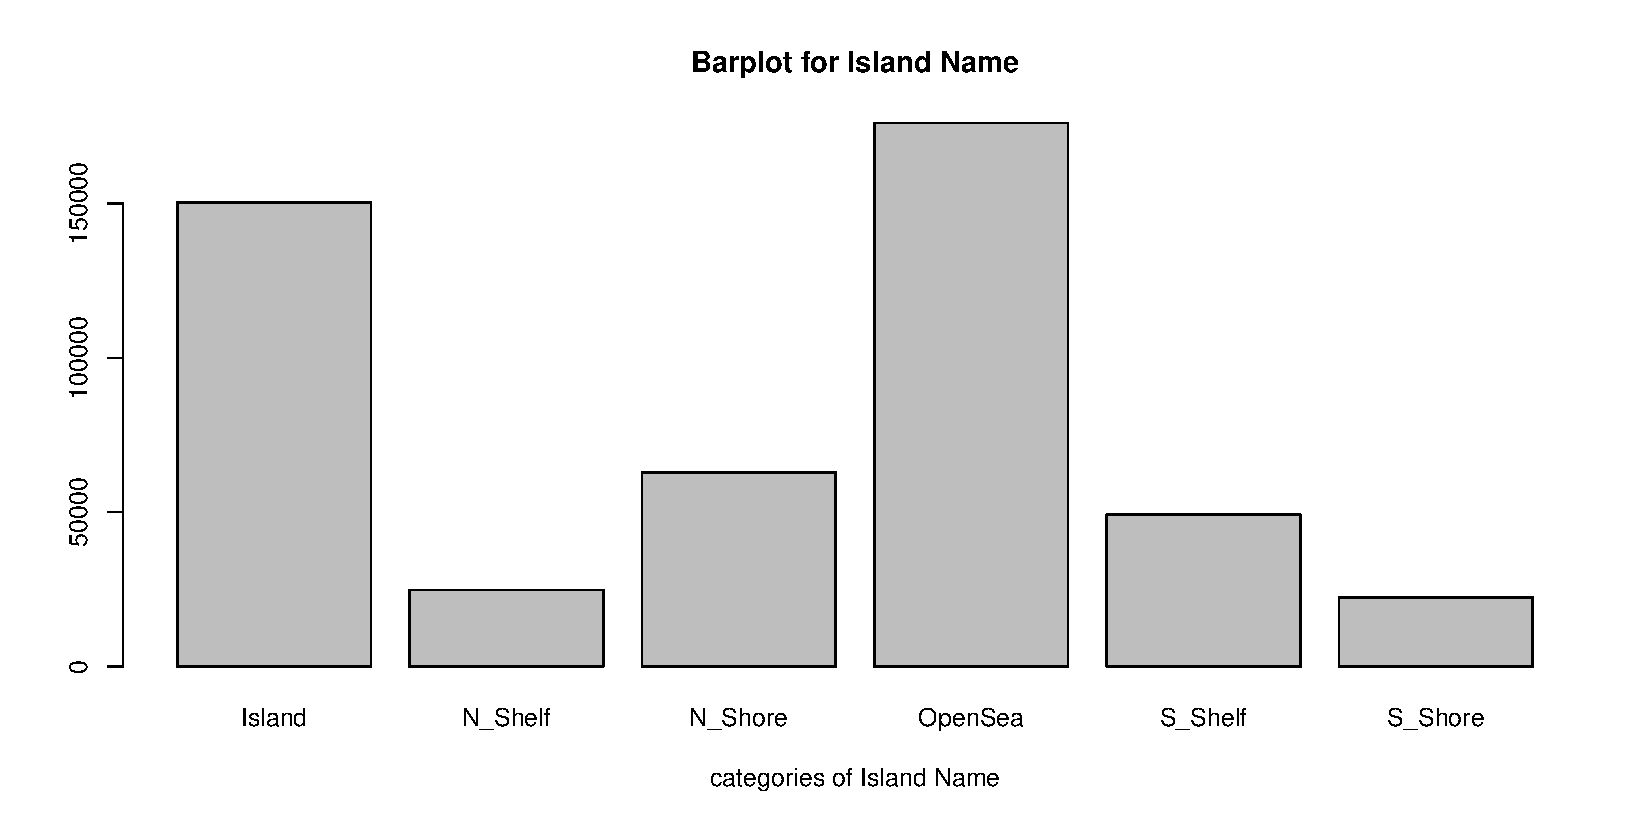
\includegraphics{Osorio_Daniel_HW3-015}
\end{enumerate}
\end{enumerate}
\end{document}
